\chapter[A Wonderful Scholar, Guide and leader in Theoretical\hfil\break Physics]{Prof.\ G. Ramachandran: A Wonderful Scholar, Guide and leader in Theoretical Physics}\label{chap35}

\Authorline{Vikas M. Shelar}
\authinfo{Ramaiah university of Applied Sciences, Bangalore}

Prof.\ G.\ Ramachandran was an internationally renowned scholar, a person with a strong opinion. The meticulous manner in which he prepared and delivered his lectures has been widely acclaimed by all his students for over six decades in India and abroad. We all will remember him for his extraordinary teaching and mentoring.

I was fortunate to have had Prof.\ G. Ramachandran as my\break co-supervisor for my Ph.D. degree at NITK Surathkal. The first time I had an opportunity to meet Prof.\ G. Ramachnadran was when I was working with ISRO Radar Development Unit. Our Group Director Sri G. Viswanathan Sir introduced me to his brother Prof.\ G. Ramachandran a great Physicist. During that short visit, I discussed a bit of Physics and became aware of his expertise in Theoretical Physics, especially electromagnetic theory and quantum theory of angular momentum. During April -- May 2008, I got a call from Prof.\ G. Ramachandran Sir and he told me that Ph.D. admission are open at NITK Surathkal. He encouraged me to apply and, subsequently, I met Prof.\ G. Umesh, who was Prof.\ Ramachandran's student in M.Sc., and he became my research supervisor at NITK. Initially we thought of working on electromagnetic theory and address the problem of polarized Electromagnetic (EM) wave scattering from non-spherical particles with the guidance of Prof.\ G. Ramachandran. We immediately realized that, in the year 1908 Lorentz and Mie had worked out the solution to the problem of EM wave scattering by spherical particles. The incident plane wave and the scattered field was expanded in terms of vector spherical harmonics. The internal field was expanded into regular vector spherical harmonics. The result was expressed as spherical polynomials. There are large number of articles and books devoted to the extension of this method to non-spherical particles. After a few months of this study, it was decided that we will work on  laser induced fluorescence spectroscopy. This had immediate applications to experiments on high speed Aerodynamics. This technique was to be tested in the Shock-Tube Facilities at Aerospace Engineering Department, Indian Institute of Science (IISc).

Prof.\ G. Ramachandran was my co-supervisor and with his help I finally wrote the first chapter of my Thesis on Fluorescence emission and its polarization characteristics. I used to meet him at Bengaluru daily for a couple of months. I used to visit his house every day to discuss the EM field theory and he always used to teach me  with the same energy as on the first discussion. We used to discuss the quantum field theoretical approach to the phenomenon of fluorescence from atoms, which had wide applications, including laser induced fluorescence. When radiation is absorbed or emitted by an atom, angular momentum and parity are conserved. Therefore the photon which is emitted or absorbed is also characterized by well-defined angular momentum quantum number L and parity. Therefore it was necessary to have complete understanding of angular momentum and parity. This became the main content in first chapter of my thesis. He not only taught me how to analyze potential problems, refined my understanding of EM theory, but also revealed how to always regard the students `wellbeing and education' as a priority. Every evening there used to be discussions and after that I used to write up what I had learnt. We also had discussions about the development of scientific thinking in the students and society.

Prof.\ G. Ramachandran was an extremely humble human being and his humility and dedication to work were exemplary. He will be remembered by all his students and colleagues as an affectionate and beloved teacher who gave his best to his students till the last day. Compassion, thoughtfulness, considerate and devoted towards students best describe him as a person. I really enjoyed working with him. I learnt a lot from him. I will forever be grateful to him for the guidance and mentorship which has impacted my life in a major way.
\vskip 1cm

\centerline{\includegraphics[scale=2]{authorsphotos/Dr_Vikas_Shelar.eps}}
\medskip

\noindent
\textbf{Dr.\ Vikas Shelar} obtained the M.Sc.\ degree in 2005 from Karnataka University and the Ph.D. degree in 2014 from NITK Surathkal.  He worked as a Research Associate for a year at Aerospace Engineering Department, I.I.Sc. Bangalore. Since 2015 he has been working as Assistant Professor in Physics Department, Ramaiah University of Applied Sciences, Bengaluru, where he is currently Academic Registrar.
